\chapter{Inteligență artificială}

\section{Recunoașterea vorbirii}
Pentru a putea recunoaște vorbirea dintr-un videoclip, am ales să folosesc arhitectura
\textit{wav2vec 2.0} \cite{wav2vec2} dezvoltată de Facebook AI Research. Am folosit 
atât modelul \textit{facebook/wav2vec2-base-960h} antrenat pe setul de date 
\textit{LibriSpeech} \cite{librispeech}, cât și modelul preantrenat
\textit{facebook/wav2vec2-base} pe care am continuat să-l antrenez pe seturile
de date \textit{Mini LibriSpeech} (subset din LibriSpeech) și
\textit{Common Voice Delta Segment 16.1} (subset din Common Voice) \cite{commonvoice}.
\par

\subsection{Arhitectura modelului}
Modelul \textit{wav2vec 2.0} este un model de învățare profundă alcătuit din 4
componente principale: Latent Feature Encoder (Convolutional Network), Context 
Network (Transformer Encoder), Quantization Module (Gumbel Softmax) și 
Contrastive Loss. \ref{fig:wav2vec2-architecture}

\begin{figure}[h]
    \centering
    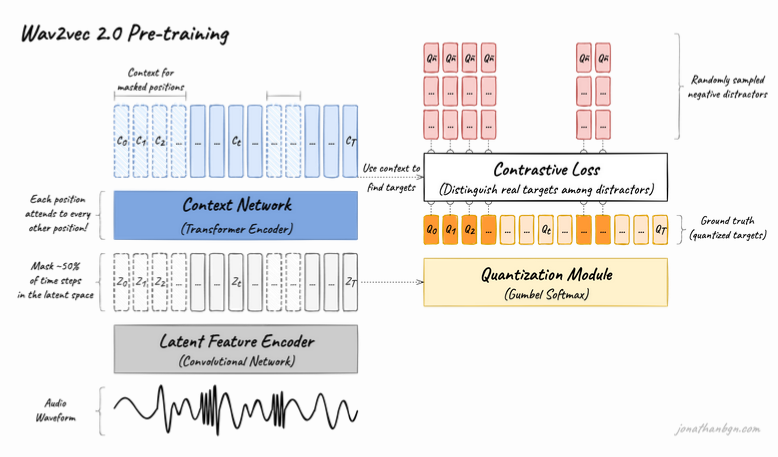
\includegraphics[width=0.8\textwidth]{wav2vec2-architecture.png}
    \caption{Arhitectura modelului \textit{wav2vec 2.0} \protect\footnotemark[1]}
    \label{fig:wav2vec2-architecture}
\end{figure}

\subsubsection{Latent Feature Encoder}
\vspace{3em}
Componenta Latent Feature Encoder este o rețea convoluțională care primește ca 
intrare un semnal audio și aplică o serie de operații de convoluție, normalizare
și activări GELU pentru a extrage caracteristici latente din semnalul audio.
\ref{fig:latent-feature-encoder}

\vspace{3em}

\begin{figure}[h]
    \centering
    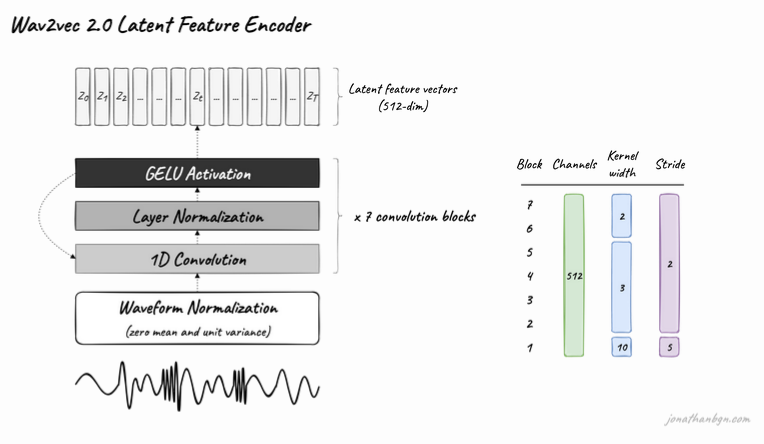
\includegraphics[width=0.8\textwidth]{wav2vec2-feature-encoder.png}
    \caption{Arhitectura componentei Latent Feature Encoder \protect\footnotemark[1]}
    \label{fig:latent-feature-encoder}
\end{figure}


\vspace{3em}

\subsubsection{Context Network}
\vspace{1em}
Componenta Context Network este un encoder de tip Transformer care primește ca
intrare caracteristicile latente extrase de componenta Latent Feature Encoder și
le procesează pentru a obține o reprezentare contextuală a semnalului audio. Aducând
aminte de arhitectura modelului anterior \textit{wav2vec} \cite{wav2vec}, care folosea
tot o rețea convoluțională la acest pas, ar părea că se aseamană cu componenta anterioară.
Diferența constă în faptul că Latent Feature Encoder urmărește să reducă dimensiunea 
semnalului audio, în timp ce Context Network urmărește să înțeleagă un context mai larg
al semnalului audio. \ref{fig:wav2vec2-context-network}

\begin{figure}[h]
    \centering
    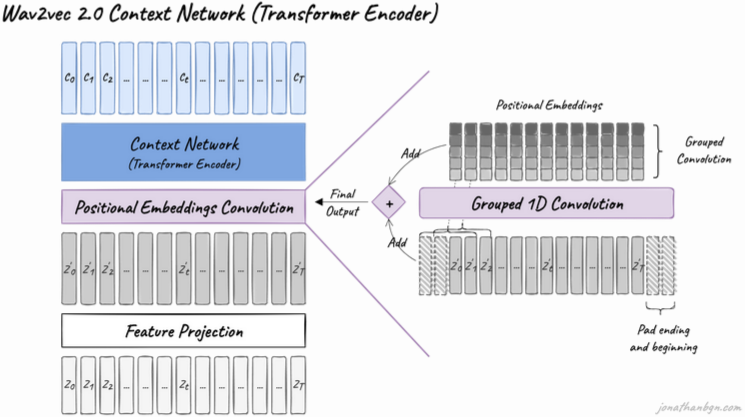
\includegraphics[width=0.8\textwidth]{wav2vec2-context-network.png}
    \caption{Arhitectura componentei Context Network \protect\footnotemark[1]}
    \label{fig:wav2vec2-context-network}
\end{figure}

\vspace{3em}

\subsubsection{Quantization Module} 
Deoarece modelul \textit{wav2vec 2.0} folosește pentru partea de Context Network un encoder de tip
Transformer, ne confruntăm cu problema structurii continue a semnalului audio. Limbajul scris poate
fi discretizat într-un set finit de simboluri, în timp ce semnalul audio nu permite în mod direct
acest lucru. Astfel, modelul \textit{wav2vec 2.0} folosește un modul de cuantizare care învață automat
unități de vorbire din semnalul audio. Intuitiv, se încearcă găsirea unor sunete fonetice 
finite și reprezentative pentru ieșirile din Latent Feature Encoder. De asemenea, se aplică 
funcția Gumbel Softmax \cite{gumbel-softmax}, funcție diferențiabilă care permite antrenarea modelului
prin backpropagation. \ref{fig:wav2vec2-quantization-module}

\begin{figure}[h]
    \centering
    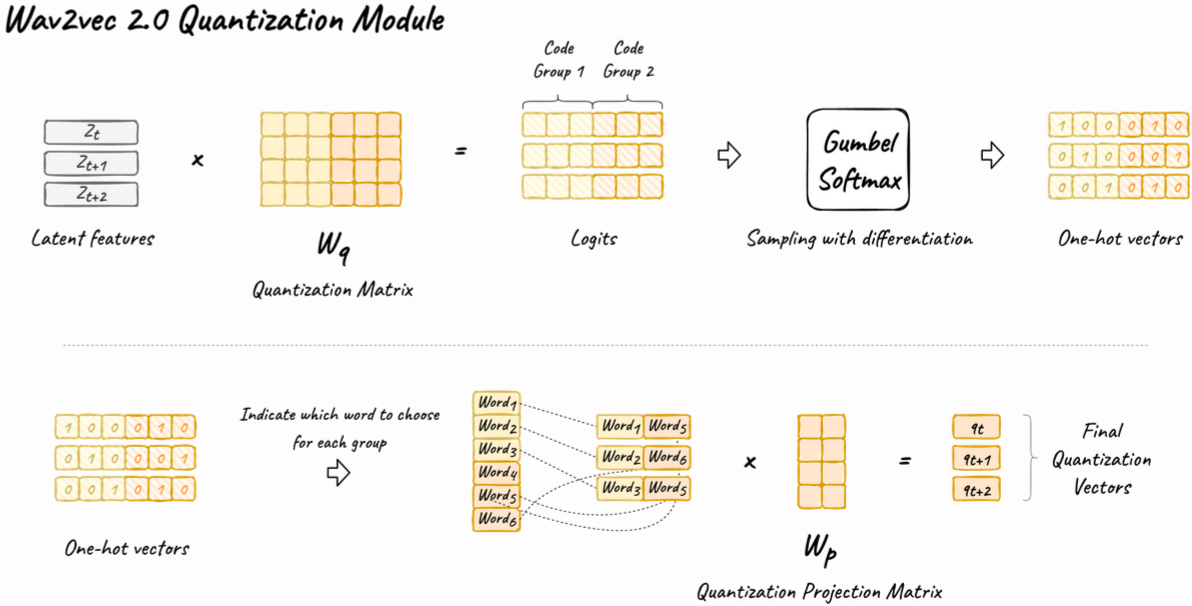
\includegraphics[width=0.8\textwidth]{wav2vec2-quantization-module.png}
    \caption{Arhitectura componentei Quantization Module \protect\footnotemark[1]}
    \label{fig:wav2vec2-quantization-module}
\end{figure}

\subsubsection{Contrastive Loss}
Pentru antrenarea modelului folosește o mască care ascunde ~50\% din vectorii proiectați din spațiul
latent înainte să fie trecuți prin Context Network. Acest lucru forțează modelul să învețe
reprezentări între vectorii proiectați și vectorii ascunși. Pentru fiecare poziție mascată, se
aleg uniform aleator 100 de exemple negative de la alte poziții și se compară similaritatea cosinus
între vectorul proiectat și vectorii aleși. Astfel, funcția de pierdere contrastivă încurajează
similaritatea cu exemplele true positive și penalizează similaritatea cu exemplele false positive.

\begin{figure}[h]
    \centering 
    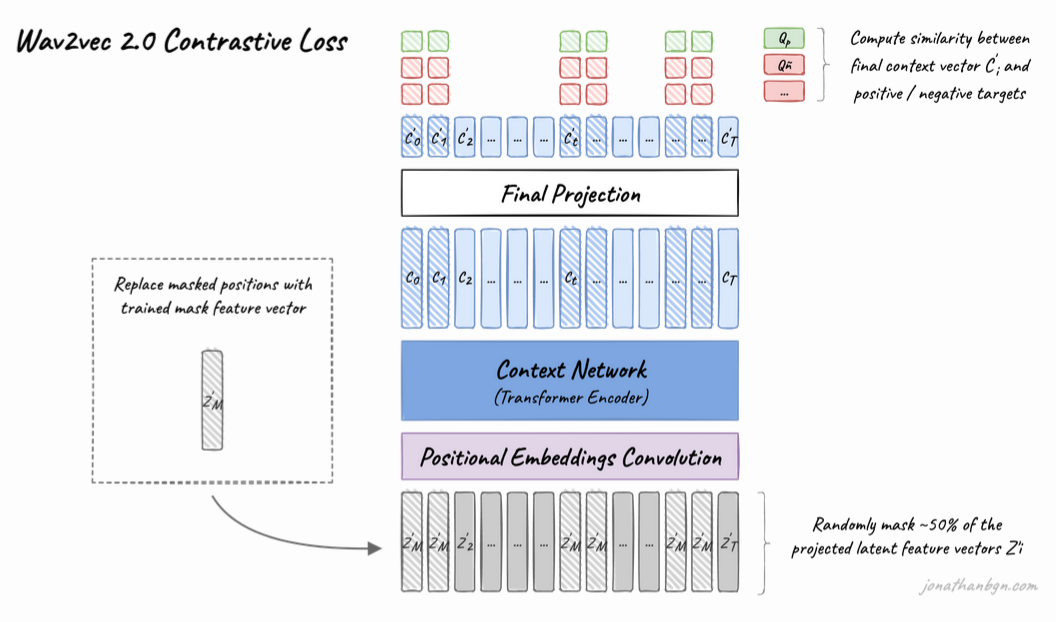
\includegraphics[width=0.8\textwidth]{wav2vec2-contrastive-loss.png}
    \caption{Arhitectura componentei Contrastive Loss \protect\footnotemark[1]}
    \label{fig:wav2vec2-contrastive-loss}
\end{figure}

\footnotetext[1]{Imaginile au fost preluate de pe site-ul lui Jonathan Bgn, ``Illustrated Wav2Vec 2.0'', disponibil la: \url{https://jonathanbgn.com/2021/09/30/illustrated-wav2vec-2.html}.}

\subsection{Setul de date}
Modelul oficial a fost preantrenat pe setul de date \textit{LibriSpeech}, iar eu am continuat
antrenarea pe seturile de date \textit{Mini LibriSpeech} și \textit{Common Voice Delta Segment 16.1}.

\subsubsection{Mini-LibriSpeech}
\textit{Mini LibriSpeech} este un subset al setului de date \textit{LibriSpeech} care conține 
aproximativ 2 ore de înregistrări audio la o frecvență de eșantionare de 16 kHz. În medie,
fiecare înregistrare are o durată de 6.72 secunde, cel mai lung audio având o durată de 31.5 secunde.

\subsubsection{Common Voice Delta Segment 16.1}
\textit{Common Voice Delta Segment 16.1} este un subset al setului de date \textit{Common Voice}
care conține aproximativ 2 ore de înregistrări audio la o frecvență de eșantionare de 48 kHz.
A fost nevoie să reduc frecvența de eșantionare la 16 kHz pentru a putea folosi aceste date la
antrenarea modelului. În medie, fiecare înregistrare are o durată de 5.63 secunde, cel mai lung
audio având o durată de 10.47 secunde.

\begin{figure}[h]
    \centering
    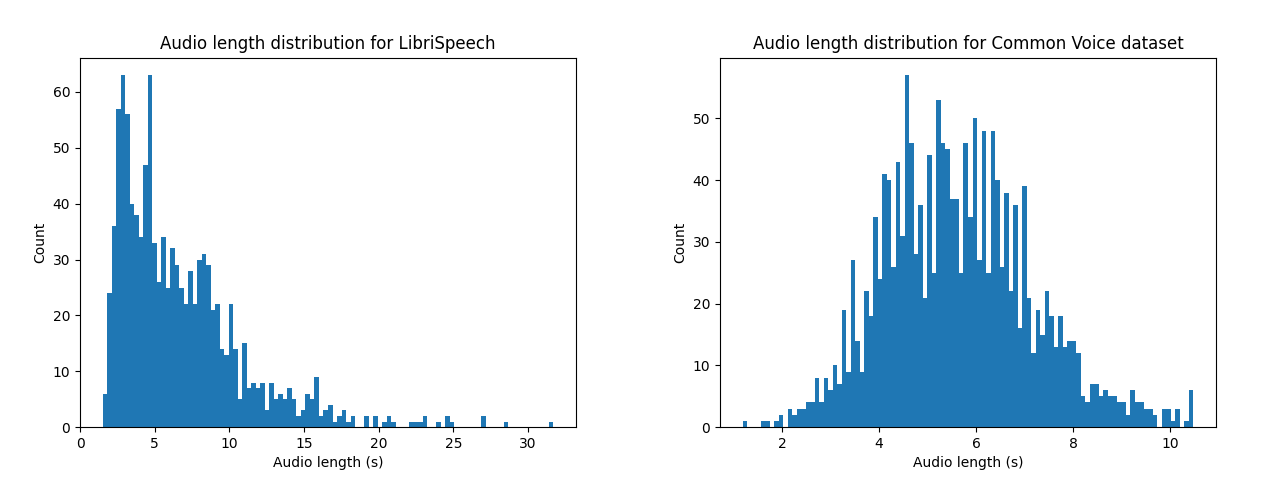
\includegraphics[width=0.8\textwidth]{length_distribution.png}
    \caption{Distribuția duratelor audio-urilor din seturile de date \textit{Mini LibriSpeech} și \textit{Common Voice Delta Segment 16.1}}
    \label{fig:length-distribution}
\end{figure}

\subsubsection{Concluzie}
Menționez aceste detalii deoarece pentru generarea subtitrărilor vom avea nevoie de audio-uri
mult mai lungi decât cele folosite pentru antrenare care nu ar încăpea în memorie. Astfel, va trebui
să folosim o tehnică de segmentare a audio-urilor în bucăți mai mici pentru a putea procesa
audio-urile mai lungi. Mai multe detalii despre această tehnică vor fi prezentate în secțiunea
\textit{Subtitări}.

\subsection{Antrenarea modelului}


\subsection{Postprocesare}
% TODO

\section{Clasificarea videoclipurilor}
% TODO

\subsection{Arhitectura modelului}
% TODO

\subsection{Setul de date}
% TODO

\subsection{Antrenarea modelului}
% TODO

\subsection{Postprocesare}
% TODO

\section{Concluzii}
% TODO
